\documentclass[11pt,a4paper]{article}
\usepackage[utf8]{inputenc}
\usepackage[T1]{fontenc}
\usepackage[spanish]{babel}
\usepackage{amsmath,amssymb}
\usepackage{booktabs}
\usepackage{array}
\usepackage{graphicx}
\usepackage{caption}
\usepackage{geometry}
\geometry{margin=2.5cm}
\usepackage{hyperref}
\hypersetup{colorlinks=true,linkcolor=blue,urlcolor=blue,citecolor=blue}

\title{Par\'ametros dependientes de temperatura\\\textit{Aedes albopictus}}
\author{Documento equivalente a \texttt{Parametros Aedes Aegypty.pdf} (modelo Yang)}
\date{}

\begin{document}
\maketitle

\noindent Documento equivalente al PDF original de \textit{Ae.\ aegypti} (modelo Yang),
adaptado para \textit{Aedes albopictus} (Skuse, 1894). Mantiene la misma estructura y
notaci\'on; los par\'ametros llevan el sub\'indice \textbf{$b$} (de \textit{albopictus})
para diferenciarlos de los de \textit{aegypti} (sub\'indice $a$).

\paragraph{Fuentes principales.}
\begin{itemize}
  \item \textbf{Delatte et al.\ (2009)}: estadio de huevo (8 reg\'imenes t\'ermicos
        constantes, cepa La R\'eunion).
  \item \textbf{Mordecai et al.\ (2017), Tabla S1}: respuestas t\'ermicas
        (Bri\`ere / cuadr\'atica) para tasas acu\'aticas y de adultos.
  \item \textbf{Marini et al.\ (2020)}: complemento para climas templados.
\end{itemize}

\section*{Funciones de respuesta t\'ermica}

Como en el documento de \textit{aegypti}, las tasas demogr\'aficas dependen de la
temperatura mediante dos formas funcionales can\'onicas:

\begin{align*}
\textbf{Bri\`ere:}\quad & f_B(T;q,T_{\min},T_{\max}) = q\,T\,(T-T_{\min})\sqrt{T_{\max}-T},
\quad T_{\min}\le T \le T_{\max} \\
\textbf{Cuadr\'atica:}\quad & f_Q(T;q,T_{\min},T_{\max}) = -q\,(T-T_{\min})(T-T_{\max}),
\quad T_{\min}\le T \le T_{\max}
\end{align*}

\noindent Ambas se anulan fuera del intervalo $[T_{\min},T_{\max}]$.

\section{Estadio de huevo (\texorpdfstring{$E_b$}{Eb})}

\begin{table}[h!]
\centering
\caption{Eclosi\'on y embriog\'enesis de \textit{Ae.\ albopictus} (Delatte et al.\ 2009).}
\begin{tabular}{rrrr}
\toprule
$T$ (\textdegree C) & $n$ huevos & $p_b$ (\%) & $\tau_b$ (d\'ias, media $\pm$ DE) \\
\midrule
5  & 180 &  4.4 & 11.0 $\pm$ 1.3 \\
10 & 100 &  4.0 &  2.0 $\pm$ 0.0 \\
15 & 110 &  8.2 &  7.4 $\pm$ 1.8 \\
20 & 130 & 66.9 &  2.9 $\pm$ 0.4 \\
25 & 130 & 49.2 &  4.5 $\pm$ 0.7 \\
30 & 140 & 51.4 &  6.7 $\pm$ 0.7 \\
35 & 190 & 10.0 &  7.1 $\pm$ 0.8 \\
40 & 100 &  0.0 & --- \\
\bottomrule
\end{tabular}
\end{table}

Tasas derivadas (siguiendo la convenci\'on del documento original):
\begin{align*}
\psi_{1b}(T) &= \frac{p_b(T)}{\tau_b(T)} \qquad \text{(tasa de eclosi\'on efectiva)} \\
\mu_{Eb}(T)  &= \frac{1-p_b(T)}{\tau_b(T)} \qquad \text{(mortalidad de huevos)}
\end{align*}

\begin{itemize}
  \item $\psi_{1b}$ m\'axima cerca de 20\,\textdegree C ($\approx 0.23$ d\'ia$^{-1}$).
  \item $\mu_{Eb}$ m\'axima a 10\,\textdegree C ($\approx 0.48$ d\'ia$^{-1}$) y a
        40\,\textdegree C, donde no hay eclosiones y se asume mortalidad total.
\end{itemize}

\paragraph{Nota sobre 10\,\textdegree C.} El valor $\tau_b = 2 \pm 0$ d\'ias en
Delatte et al.\ (2009) contradice la tendencia esperada (mayor $\tau_b$ a menor $T$).
Se mantiene la tabla tal como fue publicada; en el ajuste continuo se trata como
punto influyente menor.

\section{Estadio acu\'atico (\texorpdfstring{$L_b$}{Lb})}

\begin{align*}
\psi_{2b}(T) = \mathrm{MDR}_b(T) &= f_B(T;\,6.33\!\times\!10^{-5},\,8.7,\,39.6) \\
p_{EAb}(T) &= f_Q(T;\,3.56\!\times\!10^{-3},\,9.1,\,39.3) \\
\mu_{Lb}(T) &= \psi_{2b}(T)\left(\frac{1}{p_{EAb}(T)} - 1\right)
\end{align*}

\begin{table}[h!]
\centering
\caption{Par\'ametros t\'ermicos del estadio acu\'atico de \textit{Ae.\ albopictus} (Mordecai et al.\ 2017, Tabla S1).}
\begin{tabular}{lcrrrrl}
\toprule
Par\'ametro & Forma & $q$ & $T_{\min}$ & $T_{\max}$ & $T_{\mathrm{opt}}$ & Unidades \\
\midrule
$\mathrm{MDR}_b$ & Bri\`ere     & $6.33\!\times\!10^{-5}$ & 8.7 & 39.6 & 32.6 & d\'ia$^{-1}$ \\
$p_{EAb}$        & Cuadr\'atica & $3.56\!\times\!10^{-3}$ & 9.1 & 39.3 & 24.2 & adim. \\
\bottomrule
\end{tabular}
\end{table}

\section{Estadio adulto (\texorpdfstring{$F_b$}{Fb})}

\begin{align*}
a_b(T) &= f_B(T;\,1.90\!\times\!10^{-4},\,10.4,\,38.1) \\
\mathrm{EFOC}_b(T) &= f_B(T;\,4.77\!\times\!10^{-2},\,7.9,\,35.6) \\
lf_b(T) &= f_Q(T;\,1.39,\,13.5,\,31.4) \quad [\text{d\'ias}] \\
\phi_b(T) &= \mathrm{EFOC}_b(T)\cdot a_b(T) \\
\mu_{Fb}(T) &= \frac{1}{lf_b(T)} \\
\phi_{1b}(T) &= \frac{\sigma\,\phi_b(T)}{\mu_{Fb}(T) + \sigma}, \qquad \sigma = 1
\end{align*}

\begin{table}[h!]
\centering
\caption{Par\'ametros t\'ermicos del adulto \textit{Ae.\ albopictus} (Mordecai et al.\ 2017, Tabla S1).}
\begin{tabular}{lcrrrrl}
\toprule
Par\'ametro & Forma & $q$ & $T_{\min}$ & $T_{\max}$ & $T_{\mathrm{opt}}$ & Unidades \\
\midrule
$a_b$            & Bri\`ere     & $1.90\!\times\!10^{-4}$ & 10.4 & 38.1 & 31.8 & d\'ia$^{-1}$ \\
$\mathrm{EFOC}_b$ & Bri\`ere    & $4.77\!\times\!10^{-2}$ & 7.9  & 35.6 & 29.4 & huevos$\cdot$hembra$^{-1}\cdot$ciclo$^{-1}$ \\
$lf_b$           & Cuadr\'atica & $1.39$                  & 13.5 & 31.4 & 22.5 & d\'ia \\
\bottomrule
\end{tabular}
\end{table}

\section{Resumen comparativo \textit{aegypti} vs. \textit{albopictus}}

\begin{table}[h!]
\centering
\caption{Comparaci\'on de par\'ametros t\'ermicos (Mordecai et al.\ 2017, Tabla S1).}
\small
\begin{tabular}{llcrrr}
\toprule
Par\'ametro & Especie & Forma & $q$ & $T_{\min}$ & $T_{\max}$ \\
\midrule
\multirow{2}{*}{Tasa mordedura $a$}
  & \textit{aegypti}    & Bri\`ere & $2.02\!\times\!10^{-4}$ & 13.8 & 40.0 \\
  & \textit{albopictus} & Bri\`ere & $1.90\!\times\!10^{-4}$ & 10.4 & 38.1 \\
\midrule
\multirow{2}{*}{Fecundidad}
  & \textit{aegypti} (EFD)     & Bri\`ere & $8.16\!\times\!10^{-3}$ & 14.7 & 34.4 \\
  & \textit{albopictus} (EFOC) & Bri\`ere & $4.77\!\times\!10^{-2}$ &  7.9 & 35.6 \\
\midrule
\multirow{2}{*}{MDR}
  & \textit{aegypti}    & Bri\`ere & $7.83\!\times\!10^{-5}$ & 11.6 & 39.1 \\
  & \textit{albopictus} & Bri\`ere & $6.33\!\times\!10^{-5}$ &  8.7 & 39.6 \\
\midrule
\multirow{2}{*}{$p_{EA}$}
  & \textit{aegypti}    & Cuadr\'atica & $5.99\!\times\!10^{-3}$ & 13.6 & 38.3 \\
  & \textit{albopictus} & Cuadr\'atica & $3.56\!\times\!10^{-3}$ &  9.1 & 39.3 \\
\midrule
\multirow{2}{*}{Longevidad $lf$}
  & \textit{aegypti} (DENV) & Cuadr\'atica & $0.144$ &  9.0 & 37.7 \\
  & \textit{albopictus}     & Cuadr\'atica & $1.39$  & 13.5 & 31.4 \\
\bottomrule
\end{tabular}
\end{table}

\paragraph{Observaciones.}
\begin{enumerate}
  \item $T_{\min}$ sistem\'aticamente m\'as bajo en \textit{albopictus} salvo en
        $lf$ (donde \textit{aegypti} reporta $T_{\min} = 9.0$ pero con $q$ mucho
        menor y curva m\'as plana). Explica la expansi\'on de \textit{albopictus}
        a zonas templadas.
  \item $T_{\max}$ similar o ligeramente menor en \textit{albopictus} para $a$,
        $\mathrm{EFOC}$ y $lf$: no es m\'as tolerante al calor extremo.
  \item $lf$ en \textit{albopictus} es cualitativamente distinta: ventana
        $[13.5,31.4]$\,\textdegree C, m\'aximo en 22.5\,\textdegree C
        ($\approx 28$ d\'ias).
\end{enumerate}

\section{Figuras}

\begin{figure}[h!]
\centering
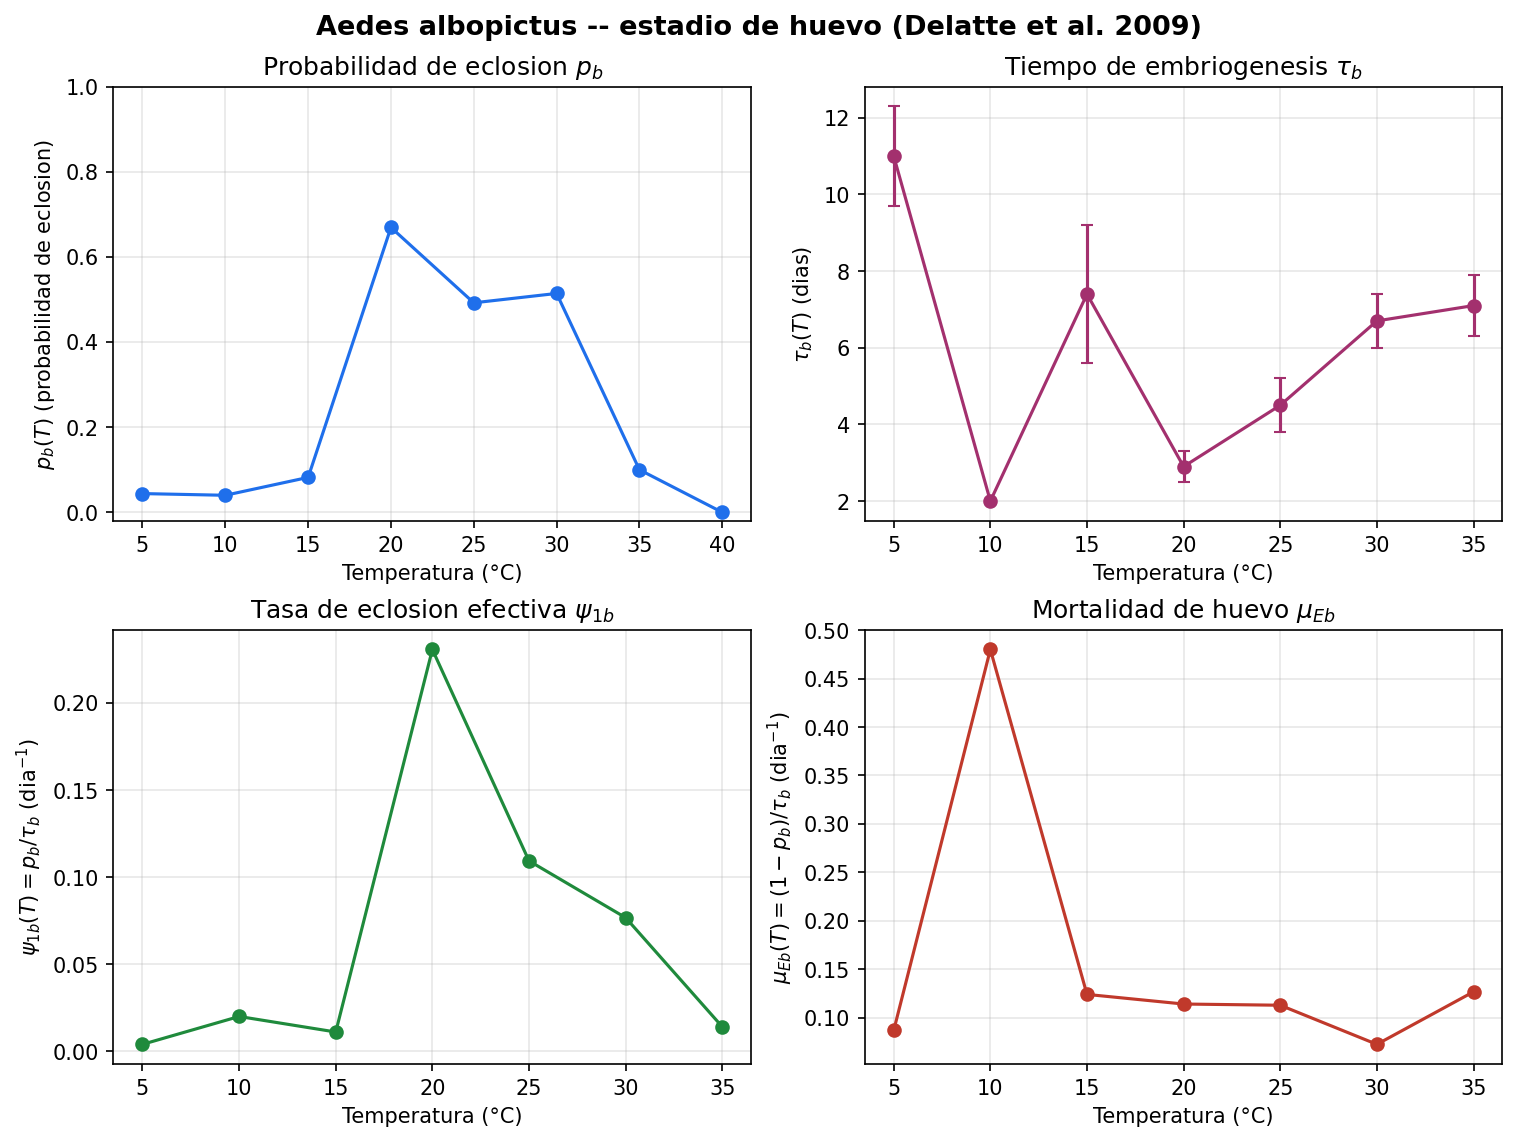
\includegraphics[width=0.85\textwidth]{figures/albopictus_egg_stage.png}
\caption{Estadio de huevo de \textit{Ae.\ albopictus}: $p_b(T)$, $\tau_b(T)$,
$\psi_{1b}(T)$ y $\mu_{Eb}(T)$ derivados de Delatte et al.\ (2009).}
\end{figure}

\begin{figure}[h!]
\centering
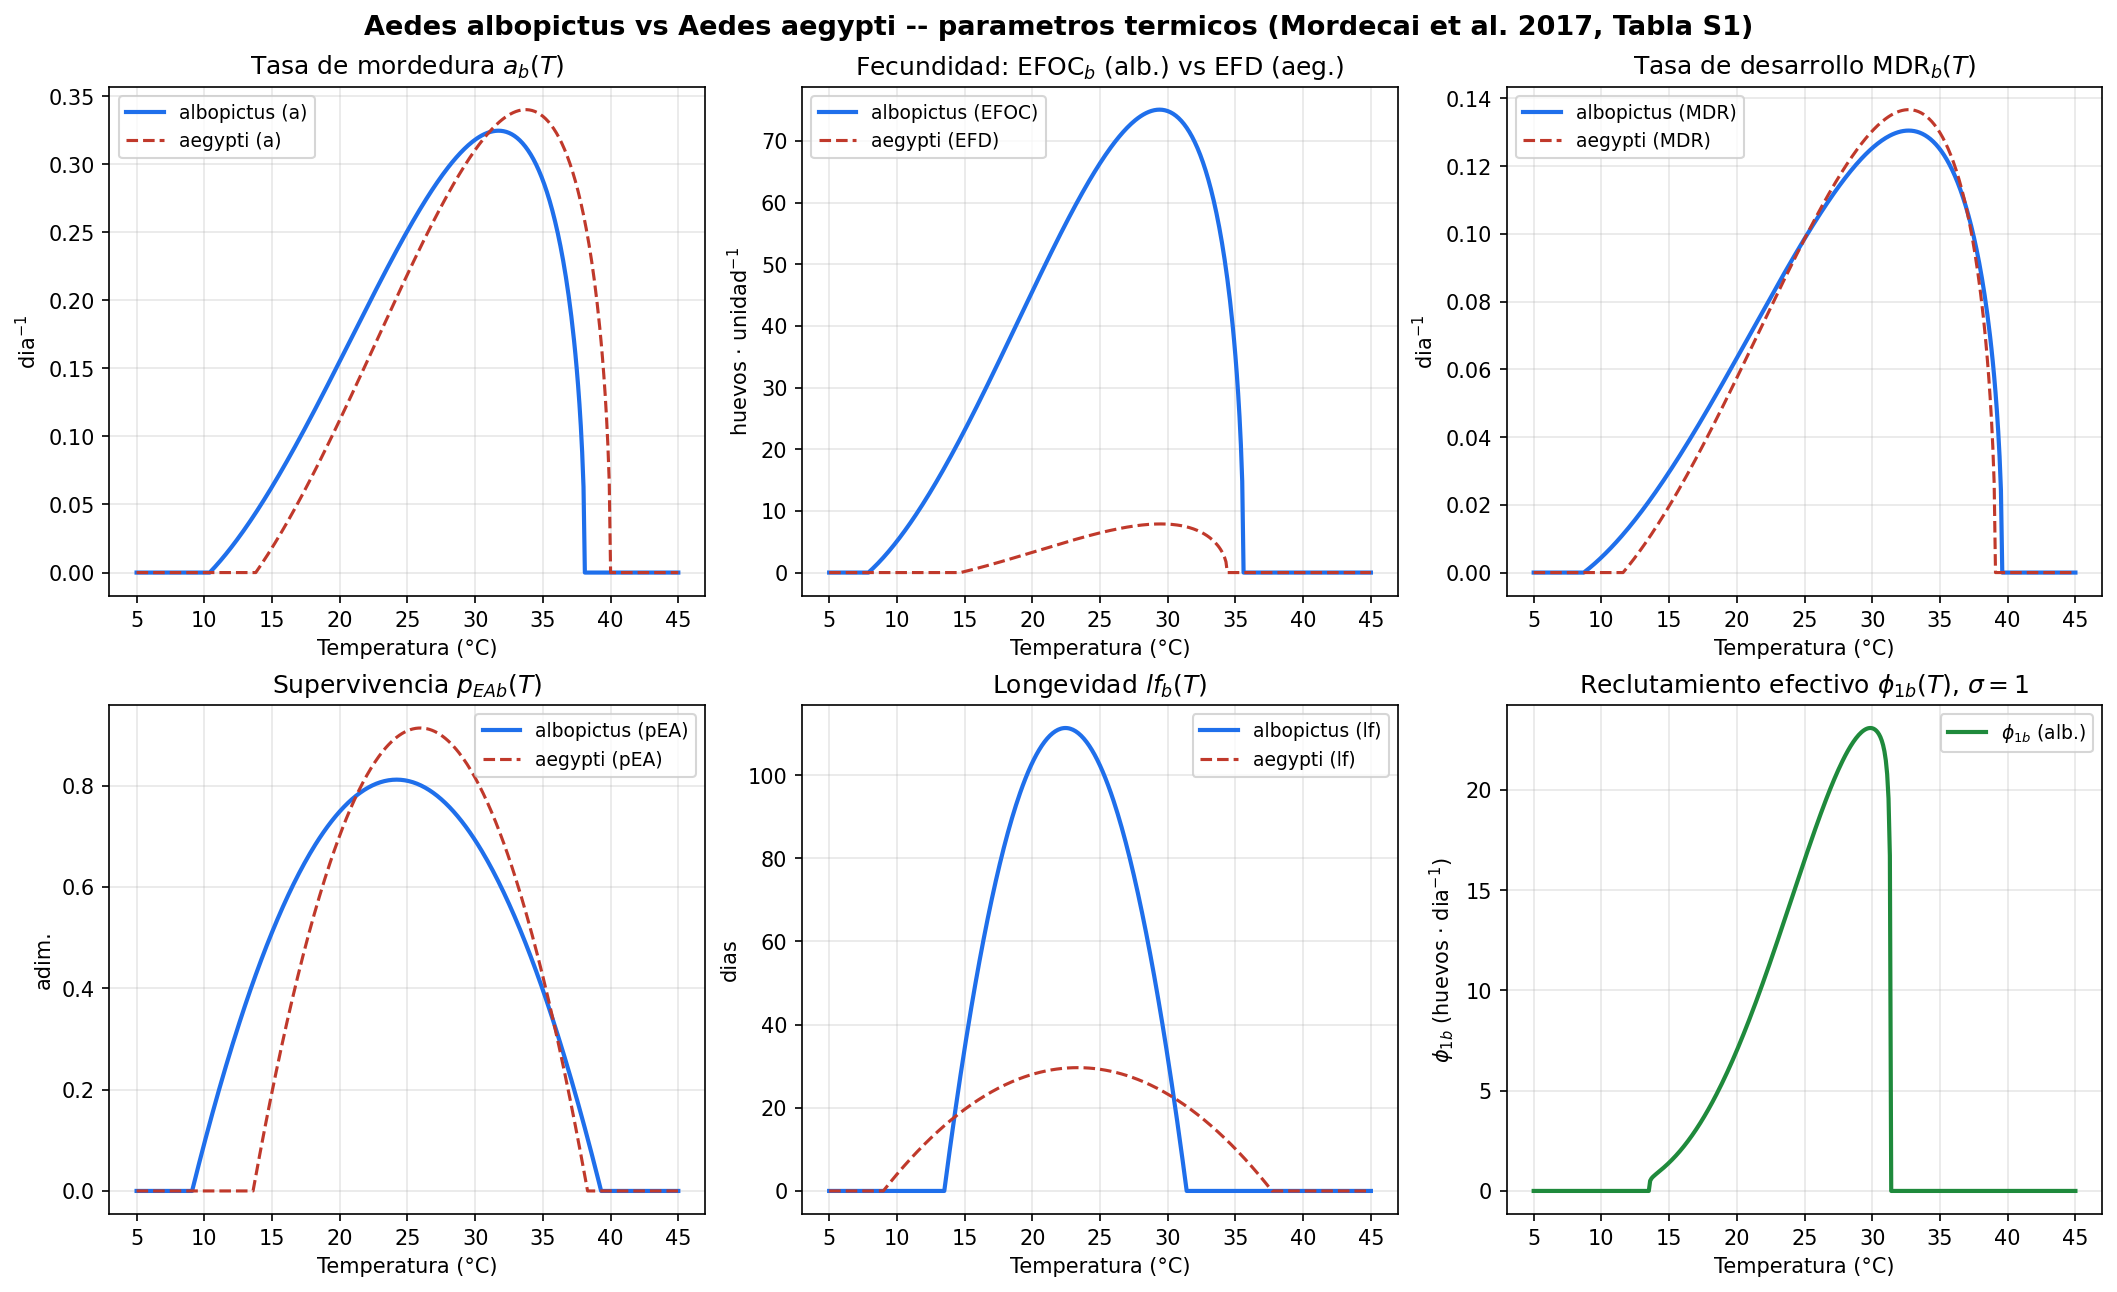
\includegraphics[width=\textwidth]{figures/albopictus_params_overview.png}
\caption{Funciones continuas de respuesta t\'ermica para \textit{Ae.\ albopictus}
(l\'inea continua) comparadas con \textit{Ae.\ aegypti} (l\'inea discontinua) en el
rango 5--45\,\textdegree C. Par\'ametros de Mordecai et al.\ (2017, Tabla S1).}
\end{figure}

\section*{Referencias}

\begin{enumerate}
  \item Delatte, H., Gimonneau, G., Triboire, A., \& Fontenille, D. (2009).
        Influence of temperature on immature development, survival, longevity,
        fecundity, and gonotrophic cycles of \textit{Aedes albopictus}, vector
        of Chikungunya and Dengue in the Indian Ocean. \textit{Journal of Medical
        Entomology}, 46(1), 33--41.
  \item Mordecai, E. A., et al.\ (2017). Detecting the impact of temperature on
        transmission of Zika, dengue, and chikungunya using mechanistic models.
        \textit{PLoS Neglected Tropical Diseases}, 11(4), e0005568. Par\'ametros
        de la \textbf{Tabla S1} del material suplementario.
  \item Marini, G., Manica, M., Delucchi, L., Pugliese, A., \& Ros\`a, R. (2020).
        Spatio-temporal distribution of \textit{Aedes albopictus} in Europe and
        its prospective range expansion under climate change. \textit{Veterinary
        Italiana}, 56(2), 109--118.
  \item Yang, H. M., et al.\ (2009). Assessing the effects of temperature on the
        population of \textit{Aedes aegypti}, the vector of dengue.
        \textit{Epidemiology and Infection}, 137(8), 1188--1202.
\end{enumerate}

\end{document}
